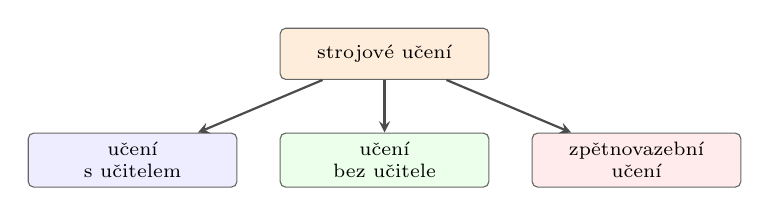
\begin{tikzpicture}[
    >=stealth,
    box/.style={
        draw=black!60,
        rounded corners=2pt,
        minimum width=2.65cm,
        minimum height=0.65cm,
        align=center,
        font=\scriptsize
    },
    arr/.style={->, thick, draw=black!70}
]
    \node[box, fill=orange!14] (ml) at (0,1.8)
        {strojové učení};

    \node[box, fill=blue!7] (sup) at (-3.2,0.45)
        {učení\\s učitelem};

    \node[box, fill=green!8] (unsup) at (0,0.45)
        {učení\\bez učitele};

    \node[box, fill=red!8] (rl) at (3.2,0.45)
        {zpětnovazební\\učení};

    \draw[arr] (ml) -- (sup);
    \draw[arr] (ml) -- (unsup);
    \draw[arr] (ml) -- (rl);
\end{tikzpicture}
